\section{Week 7}
\textbf{\underline{Pole-Zero Placement}}

When a transfer function is given,
\begin{equation*}
    G_p (z) = \frac{z-0.1}{(z-0.8)\cdot (z^2-z+0.34)} \; ,
\end{equation*}

and the question asks for a pole/zero placement that makes the system goes through a certain point that was not originally on the root locus,
\begin{equation*}
    z^* = 0.4+j\,0.17 \; ,
\end{equation*}

Do the following steps:
\begin{enumerate}
    \item Compute $G_p(z^*)$. In this example,
    \begin{align*}
        G_p(z^*) &= -1.38451 - j\, 9.3625 \\
        &= 9.46432 \, \angle -98.41^{\circ} 
    \end{align*}
    \item Obtain the angle contribution the controller needs to provide. In this case,
    \begin{align*}
        \theta &= -180^{\circ} - (-98.41^{\circ}) \\
        &= -81.58^{\circ} 
    \end{align*}
    \item Use geometry to determine the pole/zero location (not sure if there's a better and quicker way).
\end{enumerate}
\begin{figure}[h]
    \centering
    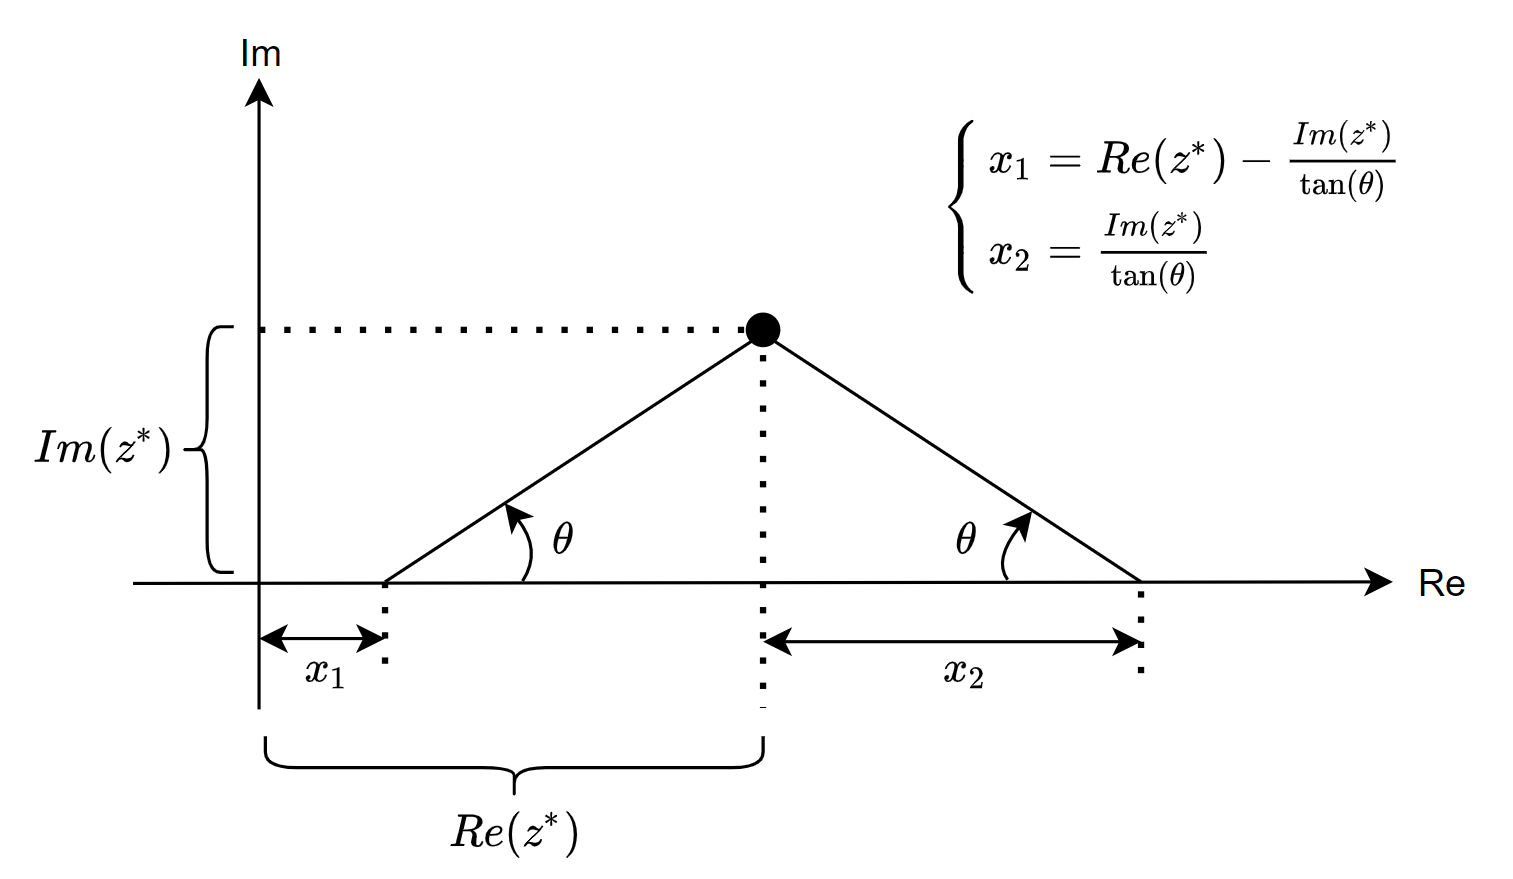
\includegraphics[width=1.0\linewidth]{images/pole_placement.png}
\end{figure}
    
\textbf{\large Cancellations:}
\begin{itemize}
    \item Cancellation of unstable poles of $G_p$ at the implementation stage leads to instability, because the value of physical poles cannot be precisely measured.
    \item Cancellation taken place at the computational plane is harmless.
    \item Cancel a pole with real parts greater than 0 in z-domain is more worrisome than cancelling a pole with negative real part.
    \begin{equation*}
        \begin{cases}
            \frac{4(z+0.5)}{(z+0.5)(z-0.1)} \\
            y(k) = C_1 (-0.5)^k + C_2 (0.1)^k
        \end{cases}
    \end{equation*}
    Ex. $(z-0.1)$ is the more worrying pole because $C_2 (0.1)^k$ is growing while $C_1 (-0.5)^k$ is neutral and ringing.
\end{itemize}
